\section{Splinter: Practical, Private Web Application Queries}
\label{chap:splinter}

\subsection{Motivation}

Web services are collecting increasing amounts
of data, and this data contains information of interest
to both users and businesses. For example,
users can access crowdsourced information,
such as the most up-to-date
traffic data to determine the fastest route.
Similarly, businesses can leverage this crowdsourced data to extract
cross-user trends that would be difficult or impossible to
detect without this data.
Many of these applications that crowdsource data 
currently allow users to query their datasets. For example, users might search
WebMD for some information on their medical condition. Similarly,
they might also search Yelp to find a restaurant for dinner.
An increasing number of web services with crowdsourced data
are also allowing businesses and researchers to query
their dataset. Google, for instance, has an API that allows
organizations to query its map data to improve business decisions.
However, the problem is that 
these queries can reveal sensitive information,
such as medical conditions, user behavior, 
and business strategy~\cite{narayanan2010myths, narayanan2008robust}.

%Many online services let users query large datasets:
%some examples include restaurant sites, stock quotes,
%medical information, and patents. In these services, 
%any user can query the data, and the datasets themselves
%do not contain sensitive user data. 
%However, web services can infer a great deal of identifiable and sensitive
%user information from these queries, such as her 
%political affiliation, sexual orientation, income,
%medical conditions, behavior, etc.~\cite{narayanan2010myths, narayanan2008robust}.
%Web services can use this information maliciously and put users at risk to practices such as
%discriminatory pricing~\cite{amazon-disc-pricing, price-disc2, hannak2014measuring}.
%For example, online stores have charged users different prices based on location~\cite{price-disc}, and
%travel sites have also increased prices for certain frequently searched flights~\cite{travel-pricing}.
%Even when the services are honest, server compromise and subpoenas can leak the sensitive user
%information collected by these services~\cite{ravichandran2009capturing, yelp-compromise, twitter-compromise}.

To solve this problem, we introduce Splinter, a practical system that allows servers
to properly respond to queries without servers learning the sensitive information 
present in the queries. In Splinter, each \emph{provider} hosts a copy of the dataset (Figure~\ref{fig:overview}).
Then, the user\footnote{In this chapter of the dissertation, we use the term "user" broadly
to refer to a business, a researcher, and end-user of an application, i.e. any client of Splinter.} 
divides each query into shares and sends them to these providers.
As long as any one of the providers is honest (does not
collude with the others), the providers cannot discover sensitive
information in the query. However, given responses from all the providers, the user
can compute the answer to her query.

\begin{figure}
	\centering
	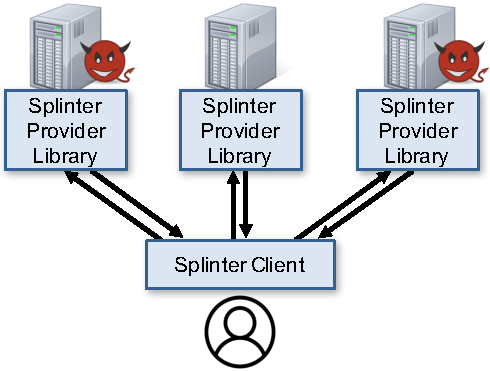
\includegraphics[width=\textwidth]{splinter-figs/overview.pdf}
	\caption[Overview of Splinter architecture.]{
		Splinter architecture. 
		The Splinter client splits each user query into shares and sends them to multiple
		providers. It then combines their results to obtain
		the final answer.
		The user's query remains private as long as any one provider does not collude with the others.
	}
	\label{fig:overview}
\end{figure}

Previous private query systems have generally not achieved practical performance
because they use expensive cryptographic primitives and protocols.
For example, systems based on techniques such
as Private Information Retrieval (PIR)~\cite{goldberg,chor1997private,pir-search} 
require many round trips and high bandwidth for complex queries, while systems based on garbled
circuits~\cite{wu2016,lan2016embark,ben2008fairplaymp} have a high computational cost.
These approaches are especially costly for mobile clients on high-latency networks.

To make private queries efficient, 
Splinter extends a recent cryptographic primitive called
Function Secret Sharing (FSS)~\cite{fss, gilboa2014distributed} for private queries.
FSS allows the client to split functions into shares that keep parameters of the
function hidden unless all the providers collude.
With judicious use of FSS, many queries can be answered in only a single network round trip
with low CPU and bandwidth costs.

Splinter extends previous work on FSS in two important ways.
First, prior work has only demonstrated efficient FSS protocols for point and interval functions with additive aggregates such as SUMs~\cite{fss}.
We present efficient protocols that support a more complex set of non-additive aggregates such as MAX/MIN and TOPK.
Together, these protocols let Splinter support a subset of SQL that can capture many popular online applications.

Second, we develop an optimized implementation of FSS that leverages AES-NI~\cite{aes-ni} instructions and multicore CPUs.
For example, we use one-way compression functions, a cryptographic technique that utilizes modern AES instruction sets. 
As a result, our implementation is 2.5$\times$ faster per core than a na\"ive implementation of FSS.
Together, these optimizations let Splinter query datasets with millions of records at sub-second latency.

We evaluate Splinter by implementing 
three applications atop it: a restaurant review site similar to Yelp, 
an airline ticket search, and a map routing service.
For all of our applications, Splinter can execute queries in less than 1.6 seconds, at a cost of less than 0.05 cents in server resources on Amazon EC2.
%Splinter's low cost means that providers could profitably run a Splinter-based service
%similar to OpenStreetMap routing~\cite{osm}, an open-source maps service, while only charging users a few dollars per month.

%Finally, Splinter does have some limitations.
%First, FSS, like PIR, requires scanning the whole input dataset on
%every query, to prevent providers from figuring out which records have
%been accessed.
%Second, Splinter does not support some SQL features, such as private join conditions.
%Despite these limitations, we show that Splinter is practical on large
%real-world datasets, such as maps, and can support many of today's online applications.
%Because human-created datasets are unlikely to grow faster than
%hardware capabilities in the future, we believe Splinter's techniques will only
%become more practical over time.

%FSS improves over PIR 
%because it allows matching \textit{multiple} records efficiently in one scan
%while practical PIR schemes can only match a single record in one scan. 
%Therefore, to the best of our knowledge,
%Splinter is the first system to practically preserve the privacy 
%of queries on large public datasets.

%In summary, our contributions are:
%\begin{itemize}
%	\item{Splinter, a private query system that achieves significantly lower CPU and communication costs than previous systems.}
%	\item{New protocols that extend FSS to complex queries with non-additive aggregates, e.g., TOPK and MAX.}
%	\item{An optimized FSS implementation for modern CPUs.}
%	\item{An evaluation of Splinter on realistic applications.}
%\end{itemize}

\subsection{Splinter Architecture}
\label{sec:goals}

In this section, we describe Splinter's principals and security goals.
Then, we discuss what services are amenable to Splinter and conclude
with the threat model.

\subsubsection{Splinter Principals}
\label{sec:model}
There are three main principals in Splinter: 
the \emph{data owners}, the \emph{providers}, and the \emph{user}.

Data owners, such as Yelp and Google, collect data, but 
they have to be comfortable releasing this data and making 
it "public." By public, we mean that the data does not
contain sensitive user information and can be stored in cleartext.

Providers host a copy of the data. They can 
retrieve this data from a public repository or mirror site,
or license it from data owners. In both scenarios,
the providers store the data in cleartext. 

Users issue queries to the provider.
For a given user query, all the providers have to execute it on the same
view of the data. Maintaining data consistency
from mirror sites is beyond the scope of this dissertation, but
standard techniques can be used~\cite{tewari2002wcdp,chi2008novel}.
%For example, OpenStreetMap~\cite{osm} publishes publicly available 
%map, point-of-interest, and traffic data. 

\subsubsection{Security Goals}
\label{sec:query_model}
The goal of Splinter is to hide sensitive parameters in
a user's query.
Specifically, Splinter lets users run \emph{parametrized queries}, 
where both the parameters and query results are hidden from providers.
For example, consider the following query, which finds the 10 cheapest flights between a source and destination:
\begin{verbatim}
SELECT TOP 10 flightid FROM flights
WHERE source = ? AND dest = ? 
ORDER BY price
\end{verbatim}
Splinter hides the information represented by the questions marks, i.e.,
the source and destination in this example.
The column names being selected and filtered are not hidden. The number 
of conditions in the WHERE clause is also not hidden.
Finally, Splinter also hides the query's results from the providers---otherwise,
the providers can use the results to infer the source and destination. 
Splinter supports a subset of the SQL language, which we describe in Section~\ref{sec:querymodel}.

The easiest way to achieve these properties would be for users to download the whole database
and run the queries locally. However, in Section~\ref{sec:splinter_cases}, we explain why
doing this might not be feasible. 

\subsubsection{Splinter-amenable Web Services}
\label{sec:splinter_cases}
Although Splinter can handle complex queries, it is not
meant as a private query system for all SQL-like databases.
Splinter's use cases are similar to those of PIR. More specifically,
the queries contain sensitive user information and need to be 
protected, but the database itself does not contain
sensitive user information. For example, users might not
want to reveal where they are traveling to Google when searching
for directions. Similarly, data analysts might want to hide
their query parameters because they might leak trade
secrets for their algorithms.

Splinter works well for applications with large databases
and regular updates because downloading the whole
database and receiving updates would be more expensive in terms
of bandwidth than querying the Splinter service. Services,
like flight price lookups, map navigation,
and domain name availability searches, are good fits for Splinter.
In Section~\ref{sec:communication}, we discuss and 
quantify the "break even" point for our case studies.

Even if it is more efficient for the user to download the whole
database and updates, Splinter can still be useful.
Many applications might enforce rate limiting or query restrictions
to prevent users from accessing the whole database
because the data might contain proprietary information.
For example, Yelp might allow only limited querying
for data scientists through an API but not give complete access to their dataset.
In this scenario, attempting a full database download would be too expensive
in comparison to employing the normal client-server query interface.

\subsubsection{Threat Model}
Splinter keeps the parameters in the user's query hidden
as long as at least one of the user-chosen providers does not collude (share information or communicate) with the others.
Splinter also assumes these providers are \textit{passive adversaries}: a provider can observe the interactions between
itself and the client, but 
Splinter does not protect against providers returning incorrect results or maliciously modifying the dataset.

We assume the data on the providers 
is stored in cleartext and that the user communicates with each provider through a secure channel (e.g., using SSL),
and that the user's Splinter client is uncompromised.
Our cryptographic assumptions are standard.

\subsection{Function Secret Sharing}
\label{sec:queries}
In this section, we give an overview of Function Secret Sharing (FSS),
the main primitive used in Splinter, and show how to use it in simple queries.
Sections~\ref{sec:querymodel} and~\ref{sec:complex} then describe Splinter's full
query model and our new techniques for more complex queries.

\subsubsection{Overview of Function Secret Sharing}
\label{sec:fss_overview}
Function Secret Sharing~\cite{fss} lets a client divide
a function $f$ into \textit{function shares} 
$f_1,f_2,\dots,f_k$ so that $k$ parties
can help evaluate $f$ without learning certain parameters.
These shares have the following properties:

\begin{itemize}
	\item{They are close in size to a description of $f$.}
	\item{They can be evaluated quickly (similar in time to $f$).}
	\item{They sum to the original function $f$.
		That is, for any input $x$, $\sum\limits_{i=1}^k f_i(x) = f(x)$. We 
		assume that all computations are done over $\mathbb{Z}_{2^m}$, 
		where $m$ is the number of bits in the output range. }
	\item{Given any $k-1$ shares $f_i$, an adversary cannot recover the parameters 
		of $f$.}
\end{itemize} 

Although it is possible to perform
FSS for arbitrary functions~\cite{dodis2016spooky}, 
practical FSS protocols only exist for \emph{point} and \emph{interval} functions.
These take the following forms:
\begin{itemize}
	\item Point functions $f_a$ are defined as $f_a(x)=1$ if $x=a$ or 0 otherwise.
	\item Interval functions are defined as $f_{a,b}(x)=1$ if $a \le x \le b$ or 0 otherwise.
\end{itemize}

In both cases, FSS keeps the parameters $a$ and $b$ private: an adversary can tell that
it was given a share of a point or interval function, but cannot find $a$ and $b$.
In Splinter, we use the FSS scheme of Boyle et al.~\cite{fss}.
Under this scheme, the shares $f_i$ for both functions require $O(\lambda \ell)$ bits to
describe and $O(\ell)$ bit operations to evaluate for a security parameter $\lambda$ (the size
of cryptographic keys), and $\ell$ is the number of bits in the input domain.

\subsubsection{Using FSS for Database Queries}
\label{sec:fss_queries}

We can use the additive nature of FSS shares to run private queries over
an entire table in addition to a single data record.
We illustrate here with two examples.

\begin{figure}
	\centering
	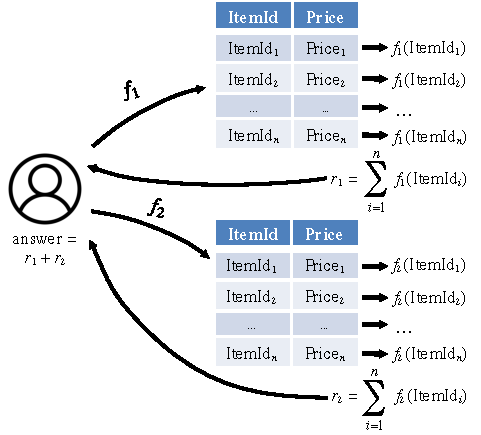
\includegraphics[width=\textwidth]{splinter-figs/fss.pdf}
	\caption{Overview of how FSS can be applied to database records
		on two providers to perform a COUNT query.}
	\label{fig:fss_overview}
\end{figure}


\paragraph{Example: COUNT query.}
Suppose that the user wants to run the following query on
a table served by Splinter:
\begin{verbatim}
SELECT COUNT(*) FROM items WHERE ItemId = ?
\end{verbatim}

Here, `\texttt{?}' denotes a parameter that the user would like to keep
private; for example, suppose the user is searching for \texttt{ItemId = 5},
but does not want to reveal this value.

To run this query, the Splinter client defines a point function $f(x)=1$ if $x=5$
or 0 otherwise.
It then divides this function into function shares $f_1,\dots,f_k$ and
distributes them to the $k$ providers, as shown in Figure~\ref{fig:fss_overview}.
For simplicity, suppose that there are two providers, who receive shares
$f_1$ and $f_2$.
Because these shares are additive, we know that $f_1(x)+f_2(x)=f(x)$
for every input $x$.
Thus, each provider $p$ can compute $f_p(\mathrm{ItemId})$ for every ItemId in the
database table, and send back $r_p = \sum_{i=1}^n f_p(\mathrm{ItemId}_i)$
to the client where $n$ is the number of database records.
The client then computes $r_1 + r_2$, which is equal
to $\sum_{i=1}^n f(\mathrm{ItemId}_i)$, that is, the count of all matching
records in the table.

\begin{figure}
	\centering
		\begin{tabular}{cccc}
			\toprule
			\bf ItemId & \bf Price & $f_1$(ItemId) & $f_2$(ItemId) \\
			\midrule
			5 & 8 & 10 & -9 \\
			1 & 8 & 3 & -3 \\
			5 & 9 & 10 & -9 \\
			\bottomrule
		\end{tabular}
	\caption[Function Secret Sharing example outputs.]{Simple example table with outputs for the FSS function shares $f_1$, $f_2$ applied to the ItemId column. 
		The function
		is a point function that returns 1 if the input is 5, and 0 otherwise.
		All outputs are integers modulo $2^m$ for some $m$.
	}
	\label{fig:fssExample2}
\end{figure}

To make this more concrete, Figure~\ref{fig:fssExample2} shows an example
table and some sample outputs of the function shares, $f_1$ and $f_2$,
applied to the ItemId column. 
There are a few important observations. First, to each provider,
the outputs of their function share seem random. Consequently, the provider does not learn
the original function $f$ and the parameter ``5''. Second, 
because $f$ evaluates 
to 1 on inputs of 5, $f_1(\mathrm{ItemId}) + f_2(\mathrm{ItemId}) = 1$ for rows 1 and 3. 
Similarly, $f_1(\mathrm{ItemId}) + f_2(\mathrm{ItemId})=0$ for row 2.
Therefore, when summed across the providers, each row
contributes 1 (if it matches) or 0 (if it does not match) to the 
final result. 
Finally, each provider aggregates the outputs of their shares by summing them. 
In the example, one provider returns 23 to the client, and
the other returns -21.
The sum of these is the correct query output, 2.

This additivity of FSS enables Splinter
to have \textit{low communication costs} for aggregate queries, by aggregating
data locally on each provider.
%Adding values locally in the provider 
%does not leak any information because each value appears random to the provider.

\paragraph{Example: SUM query.}
Suppose that instead of a COUNT, we wanted to run the following SUM query:
\begin{verbatim}
SELECT SUM(Price) FROM items WHERE ItemId=?
\end{verbatim}

This query can be executed privately with a small extension to the COUNT scheme.
As in COUNT, we define a point function $f$ for our secret predicate, e.g.,
$f(x)=1$ if $x=5$ and 0 otherwise.
We divide this function into shares $f_1$ and $f_2$.
However, instead of computing
$r_p = \sum_{i=1}^n f_p(\mathrm{ItemId}_i)$,
each provider $p$ computes
$$r_p = \sum_{i=1}^n f_p(\mathrm{ItemId}_i) \cdot \mathrm{Price}_i$$

As before, $r_1 + r_2$ is the correct answer of the query,
that is, $\sum_{i=1}^n f(\mathrm{ItemId}_i) \cdot \mathrm{Price}_i$.
We add in each row's price, $\mathrm{Price}_i$, 0 times if the ItemId is equal to 5,
and 1 time if it does not equal 5.

\subsection{Splinter Query Model}
\label{sec:querymodel}

Beyond the simple SUM and COUNT queries in the previous section, 
we have developed
protocols to execute a large class of queries using FSS, including
non-additive aggregates such as MAX and MIN, and queries that return multiple
individual records instead of an aggregate.
For all these queries, our protocols are efficient in both
computation and communication.
On a database of $n$ records, all queries can be executed in $O(n \log n)$ time
and $O(\log n)$ communication rounds, and most only require 1 or 2 communication rounds
(Figure~\ref{fig:complexity} on page~\pageref{fig:complexity}).

\begin{figure}
	%\small
	\centering
	\fbox{
		\begin{minipage}{0.7\textwidth}
			\begin{description}
				\item[\normalfont Query format:] \hspace{1mm} \\
				SELECT \emph{aggregate}$_1$, \emph{aggregate}$_2$, $\dots$ \\
				FROM \emph{table}\\
				WHERE \emph{condition}\\
				$[$GROUP BY \emph{expr}$_1$, \emph{expr}$_2$, $\dots]$
				
				\item[\normalfont \it aggregate:] \mbox{}\\[-1.5\baselineskip]
				\begin{itemize}
					\item COUNT | SUM | AVG | STDEV (\emph{expr})
					\item MAX | MIN (\emph{expr})
					\item TOPK (\emph{expr}, $k$, \emph{sort\_expr})
					\item HISTOGRAM (\emph{expr}, \emph{bins})
				\end{itemize}
				
				\item[\normalfont \it condition:] \mbox{}\\[-1.5\baselineskip]
				\begin{itemize}
					\item \emph{expr} = \emph{secret}
					\item \emph{secret}$_1$ $\le$ \emph{expr} $\le$ \emph{secret}$_2$
					\item AND of `=' conditions and up to one interval
					\item OR of multiple disjoint conditions\\
					(e.g., \texttt{country="UK" OR country="USA"})
				\end{itemize}
				
				\item[\normalfont \it expr:] any public function of the fields in a table
				row\\(e.g., \texttt{ItemId + 1} or \texttt{Price * Tax})
				
			\end{description}
		\end{minipage}
	}
	
	\caption[Splinter query format.]{Splinter query format.
		The TOPK aggregate returns the top $k$ values of \emph{expr} for matching rows
		in the query, sorting them by \emph{sort\_expr}.
		In conditions, the parameters labeled \emph{secret} are hidden from the
		providers.
	}
	\label{fig:suppq}
\end{figure}

Figure~\ref{fig:suppq} describes Splinter's supported queries using SQL syntax.
Most operators are self-explanatory.
The only exception is TOPK, which is used to return up to $k$ individual records
matching a predicate, sorting them by some expression \emph{sort\_expr}.
This operator can be used to implement \texttt{SELECT...LIMIT} queries, but
we show it as a single ``aggregate'' to simplify our exposition.
To keep the number of matching records hidden from providers, the
protocol always pads its result to exactly $k$ records.

%Note also that all queries return a bounded amount of data---there is no way to
%select arbitrarily many rows.
%This is expected given our security model: if we allowed variable-length
%results, the providers might learn something about the query from the number
%of rows sent back.

Although Splinter does not support all of SQL, we found it expressive enough to
support many real-world query services over public data.
We examined various websites, including Yelp, Hotels.com, and Kayak, and found
we can support most of their search features as shown in Section~\ref{sec:case_studies}.

Finally, Splinter only ``natively'' supports fixed-width integer data
types. However, such integers can also be used to encode strings and
fixed-precision floating point numbers (e.g., SQL DECIMALs). 
For strings in predicates, we can also encode them using hashes.
We use them to represent other types of data in our sample applications.

\subsection{Executing Splinter Queries}
\label{sec:complex}

Given a query in Splinter's query format (Figure~\ref{fig:suppq}), the system executes
it using the following steps:

\begin{enumerate}
	\item The Splinter client builds function shares for the condition in the query,
	as we shall describe in Section~\ref{sec:complex-conditions}.
	\item The client sends the query with all the secret parameters removed to
	each provider, along with that provider's share of the condition function.
	\item If the query has a GROUP BY, each provider divides its data into
	groups using the grouping expressions; otherwise, it treats the whole table
	as one group.
	\item \label{agg-step}
	For each group and each aggregate in the query, the provider runs an
	evaluation protocol that depends on the aggregate function and on
	properties of the condition. We describe these protocols in
	Section~\ref{sec:complex-aggregates}.
	Some of the protocols require
	further communication with the client, in which case the provider
	batches its communication for all grouping keys together.
\end{enumerate}

The main challenge in developing Splinter is designing efficient execution protocols
for Splinter's complex conditions and aggregates (Step~\ref{agg-step}).
Our contribution is multiple protocols that can execute non-additive
aggregates with low computation and communication costs.

One key insight that pervades our design is that \emph{the best strategy to
	compute each aggregate depends on properties of the condition function}.
For example, if we know that the condition can only match one value of
the expression it takes as input, we can simply compute the aggregate's result
for \emph{all} distinct values of the expression in the data, and then use a point
function to return just one of these results to the client.
On the other hand, if the condition can match multiple values, we need a
different strategy that can combine results across the matching values.
To reason about these properties, we define three \emph{condition classes}
that we then use in aggregate evaluation.

\subsubsection{Condition Types and Classes}
\label{sec:complex-conditions}

For any condition $c$, the Splinter client defines a function $f_c$
that evaluates to 1 on rows where $c$ is true and 0 otherwise, and divides
$f_c$ into shares for each provider.
Given a condition $c$, let $E_c = (e_1, \dots, e_t)$ be the list of
expressions referenced in $c$ (the \emph{expr} parameters in its clauses).
Because the best strategy for evaluating aggregates depends on $c$, we
divide conditions into three classes:
\begin{itemize}
	\item \emph{Single-value conditions.} These are conditions that can only be
	true on one combination of the values of $(e_1, \dots, e_t)$.
	For example, conditions consisting of an AND of `='
	clauses are single-value.
	\item \emph{Interval conditions.} These are conditions where the input
	expressions $e_1,\dots,e_t$ can be ordered such that $c$ is true on an
	interval of the range of values $e_1||e_2||\dots||e_t$ (where $||$ denotes
	string concatenation).
	\item \emph{Disjoint conditions,} i.e., all other conditions.
\end{itemize}

The condition types described in our query model (Figure~\ref{fig:suppq})
can all be converted into sharable functions, and categorized into these classes,
as follows:

\paragraph{Equality-only conditions.}
Conditions of the form
$\mathit{e}_1=\mathit{secret}_1$ AND $\dots$ AND
$\mathit{e}_t=\mathit{secret}_t$
can be executed as a single point function on the binary string
$\mathit{e}_1||\dots||\mathit{e}_t$.
This is simply a point function that can be shared using existing
FSS schemes~\cite{fss}.
These conditions are also single-value.

\paragraph{Interval and equality.}
Conditions of the form
$\mathit{e}_1=\mathit{secret}_1$ AND $\dots$ AND
$\mathit{e}_{t-1}=\mathit{secret}_{t-1}$ AND
$\mathit{secret}_{t} \le \mathit{e}_{t} \le \mathit{secret}_{t+1}$
can be executed as a single interval function on the binary string
$\mathit{e}_1||\dots||\mathit{e}_t$.
This is again supported by existing FSS schemes~\cite{fss}, and is
an interval condition.

\paragraph{Disjoint OR.}
Suppose that $c_1,\dots,c_t$ are \emph{disjoint} conditions that can be
represented using functions $f_{c_1}, \dots, f_{c_t}$.
Then $c = c_1$ OR$\dots$OR $c_t$ is captured by
$f_c = f_{c_1} + \dots + f_{c_t}$.
We share this function across providers by simply giving them shares of
the underlying functions $f_{c_i}$.
In the general case, however, $c$ is a disjoint condition where we
cannot say much about which inputs give 0 or 1.

%\footnote{
%Note also that adding the $f_i$s does not work for overlapping OR
%clauses. However, disjoint clauses are still
%useful for many real-world queries, e.g., searching for restaurants that are
%either Chinese or Indian.
%\}

\subsubsection{Aggregate Evaluation}
\label{sec:complex-aggregates}

%Our aggregate evaluation protocols depend on both the aggregate function and the
%condition class in the query.

\subsubsubsection{Sum-Based Aggregates}
To evaluate SUM, COUNT, AVG, STDEV and HISTOGRAM, Splinter
sums one or more values for each row regardless of the condition
function class.
For SUM and COUNT, each provider sums the expression being aggregated or a 1 for each
row and multiplies it by $f_i(\mathrm{row})$, its share of the condition
function, as in Section~\ref{sec:fss_queries}.
Computing AVG($x$) for an expression $x$, requires finding SUM($x$) and COUNT($x$),
while computing STDEV($x$) requires finding these values and SUM($x^2$).
Finally, computing a HISTOGRAM into bin boundaries provided by the user simply
requires tracking one count per bin, and adding each row's result to the
count for its bin. Note that the binning expression is not
private---only information about which rows pass the query's condition function.

\subsubsubsection{MAX and MIN}
\label{sec:min-max}
Suppose we are given a query to find MAX($e_0$) WHERE $c(e_1,\dots,e_t)$,
for expressions $e_0,\dots,e_t$.
The best evaluation strategy depends on the class of the condition $c$.

\paragraph{Single-value conditions.} If $c$ is only true for one combination
of the values $e_1,\dots,e_t$, each provider starts by evaluating the query
\begin{Verbatim}[commandchars=\\\{\},codes={\catcode`$=3\catcode`_=8}]
SELECT MAX($e_0$) FROM data GROUP BY $e_1,\dots,e_t$
\end{Verbatim}
This query gives an \emph{intermediate table} with the tuples $(e_1,\dots,e_t)$
as keys and $\mathrm{MAX}(e_0)$ as values.
Next, each provider computes $\sum \mathrm{MAX}(e_0) \cdot f_i(e_1,\dots,e_t)$
across the rows of the intermediate table, where $f_i$ is its share of the
condition function.
This sum will add a 0 for each non-matching row and $\mathrm{MAX}(e_0)$ for the
matching row, thus returning the right value.
Note that if the original table had $n$ rows, the intermediate table can be built
in $O(n)$ time and space using a hash table.

\paragraph{Interval conditions.}
Suppose that $c$ is true if and only if $e_1||\dots||e_t$ is in an interval $[a,b]$,
where $a$ and $b$ are secret parameters.
As in the single-value case, the providers can build a data structure that helps
them evaluate the query without knowing $a$ and $b$.
%The protocol runs as follows:

In this case, each provider builds an array $A$ of entries $(k,v)$, where the keys are all
values of $e_1||\dots||e_t$ in lexicographic order, and the values are $\mathrm{MAX}(e_0)$
for each key.
It then computes $\mathrm{MAX}(A[i..j])$ for all \emph{power-of-2 aligned} intervals
of the array $A$ (Figure~\ref{fig:complex-max-tree}).
This data structure is similar to a Fenwick tree~\cite{fenwick-trees}.

%For example, if $A$ has 6 elements, the provider will compute MAXes on
%$A[0..1]$, $A[2..3]$, $A[4..5]$ and $A[0..3]$.

\begin{figure}
	\centering
	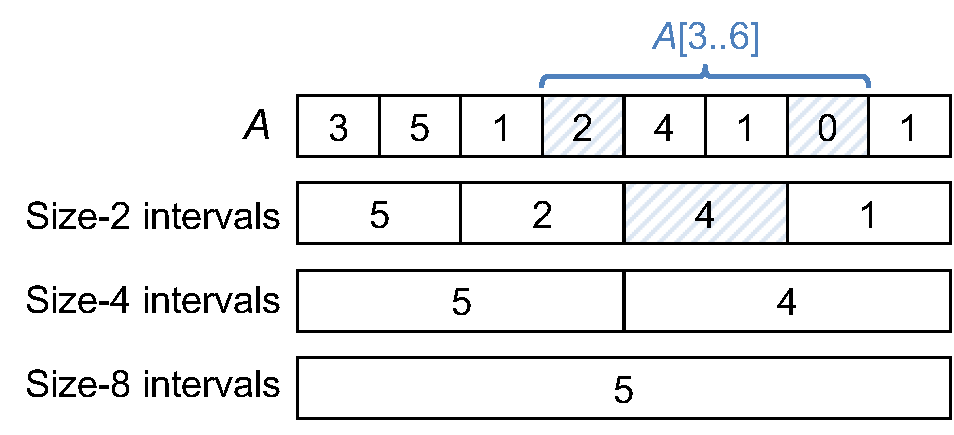
\includegraphics[width=\textwidth]{splinter-figs/complex_max_tree.pdf}
	\caption[Data structure for querying MAX on intervals.]{Data structure for querying MAX on intervals.
		We find the MAX on each power-of-2 aligned interval in the array,
		of which there are $O(n)$ total.
		Then, any interval query requires retrieving $O(\log n)$ of these
		values. For example, to find $MAX(A[3..6])$, we need two
		size-1 intervals and one size-2.
	}
	\label{fig:complex-max-tree}
\end{figure}

Query evaluation then proceeds in two rounds.
First, Splinter counts how many keys in $A$ are less than $a$ and how many are less than
$b$: the client sends the providers shares of the interval functions
$k \in [0,a-1]$ and $k \in [0,b-1]$, and the providers apply these to all keys $k$
and return their results.
This lets the client find indices $i$ and $j$ in $A$
such that all the keys $k \in [a,b]$ are in $A[i..j]$.

Second, the client sends each provider shares of new point functions that select
up to two intervals of size 1, up to two intervals of size 2, etc out of the
power-of-2 sized intervals that the providers computed MAXes on, so as to cover
exactly $A[i..j]$.
Note that any integer interval can be covered using at most 2 intervals of each power of 2.
The providers evaluate these functions to return the MAXes for the selected intervals,
and the client combines these $O(\log n)$ MAXes to find the overall MAX on $A[i..j]$.\footnote{
	To hide which sizes of intervals were actually required, the client should always request 2 intervals
	of each size and ignore unneeded ones.
}

For a table of size $n$, this protocol requires $O(n \log n)$ time at each provider
(to sort the data to build $A$, and then to answer $O(\log n)$ point function queries).
It also only requires two communication rounds, and $O(\log n)$ communication bandwidth.
The same protocol can be used for other associative aggregates, such as products.

\paragraph{Disjoint conditions.}
If we must find MAX($e_0$) WHERE $c(e_1,\dots,e_t)$ but know nothing about $c$,
Splinter builds an array $A$ of all rows in the dataset sorted by $e_0$.
Finding MAX($e_0$) WHERE $c$ is then equivalent to finding the largest index $i$
in $A$ such that $c(A[i])$ is true.
To do this, Splinter uses binary search.
The client repeatedly sends private queries of the form
\begin{Verbatim}[commandchars=\\\{\},codes={\catcode`$=3\catcode`_=8}]
SELECT COUNT(*) FROM $A$
WHERE $c(e_1,\dots,e_t)$ AND $\mathit{index}\in[\mathit{secret}_1,\mathit{secret}_2],$
\end{Verbatim}
where \textit{index} represents the index of each row in $A$ and the interval for it is kept
private. 
%(We shall discuss how to do this.)
By searching for secret intervals in decreasing power-of-2 sizes, the client can find the
largest index $i$ such that $c(A[i])$ is true.
For example, if we had an array $A$ of size 8 with largest matching element at $i=5$,
the client would probe $A[0..3]$, $A[4..7]$, $A[4..5]$, $A[6..7]$ and finally $A[4]$ to
find that 5 is the largest matching index.

Normally, ANDing the new condition $\mathit{index}\in[\mathit{secret}_1,\mathit{secret}_2]$
with $c$ would cause problems, because the resulting conditions might no longer be in
Splinter's supported condition format (ANDs with at most one interval and ORs of
disjoint clauses).
Fortunately, because the intervals in our condition are always power-of-2 aligned,
it can also be written as an equality on the first $k$ bits of \emph{index}.
For example, supposing that \emph{index} is a 3-bit value, the condition
$\mathit{index} \in [4,5]$ can be written as $\mathit{index}_{0,1} =$ ``10'', where
$\mathit{index}_{0,1}$ is the first two bits of \emph{index}.
This lets us AND the condition into all clauses of $c$.

Once the client has found the largest matching index $i$, it runs one
more query with a point function to select the row with $index = i$.
The whole protocol requires $O(\log n)$ communication rounds
and $O(n \log n)$ computation and works well if $c$ has many conditions. 

However, if $c$ has a small number of OR clauses, an optimization is to run
one query for each clause in parallel. The user then resolves
the responses locally to find the answer to the original query.
Although doing this optimization requires more bandwidth because the returned
result size is larger, it avoids the $O(\log n)$ communication rounds and 
the $O(n\log n)$ computation.

\subsubsubsection{TOPK}
\label{sec:topk}
Our protocols for evaluating TOPK are similar to those for MAX and MIN.
Suppose we are given a query to find TOPK($e$, $k$, $e_\mathrm{sort}$) WHERE $c(e_1,\dots,e_t)$.
The evaluation strategy depends on the class of the condition $c$.

\paragraph{Single-value conditions.} If $c$ is only true for one combination
of $e_1,\dots,e_t$, each provider starts by evaluating
\begin{Verbatim}[commandchars=\\\{\},codes={\catcode`$=3\catcode`_=8}]
SELECT TOPK($e,$ $k,$ $e_\mathrm{sort}$) FROM data
GROUP BY $e_1,\dots,e_t$
\end{Verbatim}
This gives an intermediate table with the tuples $(e_1,\dots,e_t)$
as keys and TOPK$(\cdot)$ for each group as values, from which we can select
the single row matching $c$ as in MAX.

\paragraph{Interval conditions.}
Here, the providers build the same auxiliary array $A$ as
in MAX, storing the TOPK for each key instead.
They then compute the TOPKs for power-of-2 aligned intervals in this array.
The client finds the interval $A[i..j]$ it needs to query, extracts the top $k$ values
for power-of-2 intervals covering it, and finds the overall top $k$.
As in MAX, this protocol requires 2 rounds and $O(\log n)$ communication bandwidth.

\paragraph{Disjoint conditions.}
Finding TOPK for disjoint conditions is different from MAX because we need to return
multiple records instead of just the largest record in the table that matches $c$.
This protocol proceeds as follows:
\begin{enumerate}
	\item The providers sort the whole table by $e_\mathrm{sort}$ to create an auxiliary array $A$.
	\item The client uses binary search to find indices $i$ and $j$ in $A$ such that the top $k$
	items matching $c$ are in $A[i..j]$. This is done the same way as in MAX, but searching for
	the largest indices where the count of later items matching $c$ is 0 and $k$.
	\item The client uses a sampling technique (Section~\ref{sec:sampling}) to extract
	the $k$ records from $A[i..j]$ that match $c$. Intuitively, although we do not know which rows
	these are, we build a result table of $>k$ values initialized to 0, and add the FSS share
	for each row of the data to one row in the result
	table, chosen by a hash. This scheme extracts all matching
	records with high probability.
\end{enumerate}
This protocol needs $O(\log n)$ communication rounds
and $O(n \log n)$ computation if there are many clauses, but like the protocol for MAX,
if the number of clauses in $c$ is small,
the user can issue parallel queries for each clause to reduce the communication rounds
and computation.

\subsubsection{Extracting Disjoint Records with FSS}
\label{sec:sampling}

Here, we describe our sampling-based technique for returning multiple records using FSS, used in TOPK queries with disjoint conditions (Section~\ref{sec:topk}).
Given a table $T$ of records and a condition $c$ that matches up to $k$ records, we wish to return those records to the client with high probability without revealing $c$.

To solve this problem, the providers each create a result table $R$ of size $l > k$, containing (value, count) columns all initialized to 0.
They then iterate through the records and choose a result row to update for each record based on a hash function $h$ of its index $i$.
For each record $r$, each provider adds $1 \cdot f_c(r)$ to $R[h(i)]$.count
and $r \cdot f_c(r)$ to $R[h(i)]$.value, where $f_c$ is its share of the condition $c$.
The client then adds up the $R$ tables from all the providers to build up a single table,
which contains a value and count for all indices that a record matching $c$ hashed into.

Given this information, the client can tell how many records hashed into each
index: entries with count=1 have only one record, which can be read from the entry's value.
Unfortunately, entries with higher counts hold multiple records that were added together in
the value field.
To recover these entries, the client can run the same process multiple times in parallel with
different hash functions $h$.

In general, for any given value of $r$ and $k$, the probability of a given record colliding with another under each hash function is a constant (e.g., it is less than $1/3$ for $r=3k$).
Repeating this process with more hash functions causes the probability to fall exponentially.
Thus, for any $k$, we can return all the distinct results with high probability using only $O(\log k)$
hash functions and hence only $O(\log k)$ extra communication bandwidth.

\subsubsection{Complexity}

\begin{figure}
	\centering
		\begin{tabular}{ccccc}
			\toprule
			\bf Aggregate & \bf Condition & \bf Time & \bf Rounds & \bf Bandwidth \\
			\midrule
			Sum-based & any & $O(n)$ & $1$ & $O(1)$ \\
			\midrule
			MAX/MIN & 1-value & $O(n)$ & $1$ & $O(1)$ \\
			MAX/MIN & interval & $O(n \log n)$ & $2$ & $O(\log n)$ \\
			MAX/MIN & disjoint & $O(n \log n)$ & $O(\log n)$ & $O(\log n)$ \\
			\midrule
			TOPK & 1-value & $O(n)$ & $1$ & $O(1)$ \\
			TOPK & interval & $O(n \log n)$ & $2$ & $O(\log n)$ \\
			TOPK & disjoint & $O(n \log n)$ & $O(\log n)$ & $O(\log n)$ \\
			\bottomrule
		\end{tabular}
	\caption[Complexity of Splinter's query evaluation protocols.]{Complexity of Splinter's query evaluation protocols for a database of size $n$.
		For bandwidth, we report the multiplier over the query's normal result size.
	}
	\label{fig:complexity}
\end{figure}

Figure~\ref{fig:complexity} summarizes the complexity of Splinter's query evaluation protocols
based on the aggregates and condition classes used.
We note that in all cases, the computation time is $O(n \log n)$ and the communication costs
are smaller than the size of the database.
This makes Splinter practical even for databases with millions of records, which covers
many common web application datasets, as shown in Section~\ref{sec:evaluation}.
Finally, the main operations used to evaluate Splinter queries at providers, namely sorting
and sums, are highly parallelizable.

\subsection{Optimized FSS Implementation}
\label{sec:fastfss}

Apart from introducing new protocols to evaluate complex queries using FSS,
Splinter includes an FSS implementation optimized for modern hardware.

The two-party FSS protocol~\cite{fss} is efficient
because of its use of one-way functions.
A common class of one-way functions is 
pseudorandom generators (PRGs)~\cite{levin1987one}, 
and in practice, 
AES is the most commonly used PRG because of hardware accelerations,
i.e. the AES-NI~\cite{aes-ni} instruction. 
Generally, using AES as a PRG is straightforward (use
AES in counter mode). However, the use of PRGs 
in FSS is not only atypical, but it also represents a large portion
of the computation cost in the protocol. The FSS protocol 
requires many instantiations 
of a PRG with different initial seed 
values, especially in the two-party 
protocol~\cite{fss}. Initializing multiple PRGs with
different seed values is very 
computationally expensive because AES cipher
initialization is \textit{much slower} than performing
an AES evaluation on an input. Therefore, 
the challenge in Splinter is to find an efficient PRG
for FSS.

Our solution is to use \textit{one-way compression functions}.
One way compression functions are commonly used as a primitive
in hash functions, like SHA, and are built using a block
cipher like AES. In particular, Splinter uses the Matyas-Meyer-Oseas one-way 
compression function~\cite{matyas1985} because
this function utilizes a \textit{fixed key} cipher. As a result, 
the Splinter protocol initializes the cipher only once per query.

More precisely, the Matyas-Meyer-Oseas one-way compression
function is defined as:
\begin{equation*}
F(x) = E_k(x) \oplus x
\end{equation*}
where $x$ is the input, i.e. PRG seed value, and $E$ is a block cipher with a fixed key $k$.

The output of a one-way compression function 
is a fixed number of bits, but we can
use multiple one-way compression functions with
different keys and concatenate the outputs to obtain more bits.
Security is preserved because a function that
is a concatenation of one-way functions is still a one-way function.

With this one-way compression function, Splinter initializes the cipher, $E_k$,
at the beginning of the query and reuses it
for the rest of the query, avoiding
expensive AES initialization operations in the FSS protocol. 
For each record, the Splinter protocol 
needs to perform only $n$ XORs and $n$ AES
evaluations using the AES-NI instruction, where
$n$ is the input domain size of the record. 
In Section~\ref{sec:micro}, we show that Splinter's use of one-way compression functions
results in a 
$2.5\times$ speedup over using AES directly as a PRG.

\subsection{Implementation}
\label{sec:implementation}

We implemented Splinter in C++, using OpenSSL 1.0.2e~\cite{openssl} 
and the AES-NI hardware instructions
for AES encryption. We used 
GMP~\cite{gmp} for large integers and OpenMP~\cite{openmp} for multithreading.
Our optimized FSS library is about 2000 lines of code, and the applications on top of it are about 2000 lines of code. There is around 
1500 lines of test code to issue the queries. 
%For comparison, 
%we also implement the multi-party
%FSS scheme in~\cite{corrigan-gibbs:riposte} using 2048 bit Paillier encryption ~\cite{paillier}.
Our FSS library implementation can be found at \url{https://github.com/frankw2/libfss}.

\subsection{Evaluation}
\label{sec:evaluation}

\begin{figure*}
	\centering
	\scalebox{0.68}{
		\begin{tabular}{llllp{1cm}p{2cm}p{2cm}p{1.5cm}}
			%\multicolumn{8}{c}{Summary of results for Splinter} \\
			\toprule
			\bf Dataset & \bf Query Desc. & \bf FSS Scheme & \bf Input Bits & \bf Round Trips & \bf Query Size & \bf Response Size & \bf Response Time \\
			\midrule
			\multirow{2}{*}{Restaurant} & \multirow{2}{*}{\parbox{4cm}{COUNT of Thai restaurants (Q1)}} & Two-party & \multirow{2}{*}{11}  & \multirow{2}{*}{1} & \textasciitilde 2.75 KB & \textasciitilde 0.03 KB & 57 ms \\
			& & Multi-party & & & \textasciitilde 10 KB & \textasciitilde 18 KB & 52 ms \\
			\midrule
			\multirow{2}{*}{Restaurant} & \multirow{2}{*}{\parbox{4cm}{Top 10 Mexican restaurants near user (Q2)}} & Two-party & \multirow{2}{*}{22}  & \multirow{2}{*}{1} & \textasciitilde 16.5 KB & \textasciitilde 7 KB & 150 ms \\
			& & Multi-party & & & \textasciitilde 1.9 MB & \textasciitilde 0.21 KB & 542 ms \\
			\midrule
			\multirow{2}{*}{Restaurant} & \multirow{2}{*}{\parbox{4cm}{Best rated restaurant in category subset (Q3)}} & Two-party & \multirow{2}{*}{11}  & \multirow{2}{*}{11} & \textasciitilde 244 KB & \textasciitilde 0.7 KB & 1.3 s \\
			& & Multi-party & & & \textasciitilde 880 KB & \textasciitilde 396 KB & 1.6 s \\
			\midrule
			\multirow{2}{*}{Flights} & \multirow{2}{*}{\parbox{4cm}{AVG monthly price for a certain flight route (Q1)}} & Two-party & \multirow{2}{*}{17} & \multirow{2}{*}{1} & \textasciitilde 8.5 KB & \textasciitilde 0.06 KB & 1.0 s \\
			& & Multi-party & & & \textasciitilde 160 KB & \textasciitilde 300 KB & 1.2 s \\
			\midrule
			\multirow{2}{*}{Flights} & \multirow{2}{*}{\parbox{4cm}{Top 10 cheapest flights for a route (Q2)}} & Two-party & \multirow{2}{*}{13} & \multirow{2}{*}{1} & \textasciitilde 3.25 KB & \textasciitilde 0.3 KB & 30 ms \\
			& & Multi-party & & & \textasciitilde 20 KB & \textasciitilde 0.13 KB & 39 ms \\
			\midrule
			\multirow{2}{*}{Maps} & \multirow{2}{*}{\parbox{4cm}{Routing query on NYC map}} & Two-party & Grid: 14 & \multirow{2}{*}{2} & \textasciitilde 12.5 KB & \textasciitilde 31 KB & 1.2 s \\
			& & Multi-party & Transit Node: 22 & & \textasciitilde 720 KB & \textasciitilde 1.1 KB & 1.0 s \\
			\bottomrule
		\end{tabular}
	}
	\caption[Performance results for Splinter case studies.]{Performance of various queries in our case study applications on Splinter. 
		Response times include 14 ms network latency per network round trip. All subqueries are issued in parallel
		unless they depend on a previous subquery. Query and response sizes are measured per provider. For the multi-party FSS scheme, we run 3 parties.
		Input bits represent the number of bits in the input domain for FSS, i.e., the maximum size of a column value.}
	\label{fig:big-results}
\end{figure*}

We built and evaluated clones of three applications 
on Splinter: Yelp clone, flight price lookup, and map routing, using real datasets.
We also compared Splinter to previous private systems, and estimate hosting costs.
Our providers ran on 64-core Amazon EC2 \texttt{x1} servers with Intel Xeon E5-2666 Haswell processors and 1.9 TB 
of RAM. The client was a 2 GHz Intel Core i7 machine with 8 GB of RAM.
Our client's network latency to the providers was 14 ms.

Overall, our experiments show the following: 
\begin{itemize}
	\item{Splinter can support realistic applications including the search features of Yelp and flight search sites, and data structures
		required for map routing.}
	\item{Splinter achieves end-to-end latencies below 1.6 seconds for queries in these applications on realistic data.}
	\item{Splinter's protocols have fewer round trips, lower bandwidth, and lower server-side computation costs than prior systems.}
\end{itemize}


\subsubsection{Case Studies}
\label{sec:case_studies}

\begin{figure}
	\centering
		\begin{tabular}{cccc}
			\toprule
			\bf Dataset & \bf \# of rows & \bf Size (MB) & \bf Cardinality \\
			\midrule
			Yelp~\cite{yelp-data} & 225,000 & 23 & 900 categories \\
			\midrule
			Flights~\cite{enigma} & 6,100,000 & 225 & 5000 flights \\
			\midrule
			\multirow{2}{*}{NYC Map~\cite{dimacs}} & 260,000 nodes & \multirow{2}{*}{300} & \multirow{2}{*}{1333 transit nodes}\\
			& 733,000 edges & \\
			\bottomrule
		\end{tabular}
	\caption[Datasets used in the evaluation.]{Datasets used in the evaluation. The cardinality of queried columns affects the input bit size in our FSS queries.}
	\label{fig:datasets}
\end{figure}

Here, we discuss the three application clones
we built on Splinter. Figure~\ref{fig:big-results}
summarizes our results, and Figure~\ref{fig:datasets}
describes the sizes and characteristics of our three datasets.
Finally, we also review the search features available in real websites
to study how many Splinter supports.

\paragraph{Restaurant review site:}
We implement a restaurant review site using the Yelp academic dataset~\cite{yelp-data}.
The original dataset contains information for local businesses in 10 cities, 
but we duplicate the dataset 4 times so that it would approximately represent
local businesses in 40 cities.
We use the following columns in the data
to perform many of the queries expressible on Yelp:
name, stars, review count, category, neighborhood and location.
%s, hex-1mi, hex-2mi, hex-5mi.
%A business might be classified into multiple categories, so there are multiple rows
%for each business (one for each category). 

For location-based queries, 
e.g., restaurants within 5 miles of a user's current location, 
multiple interval conditions on the longitude 
and latitude would typically be used. 
To run these queries faster, we quantize the locations of each restaurant into
overlapping hexagons of different radii (e.g., 1, 2 and 5 miles), following
the scheme from~\cite{narayanan2011location}.
We precompute which hexagons each restaurant is in and expose these as
additional columns in the data (e.g., \texttt{hex1mi} and \texttt{hex2mi}).
This allows the location queries to use `=' predicates instead of intervals.

%\begin{figure}
%  \centering
%     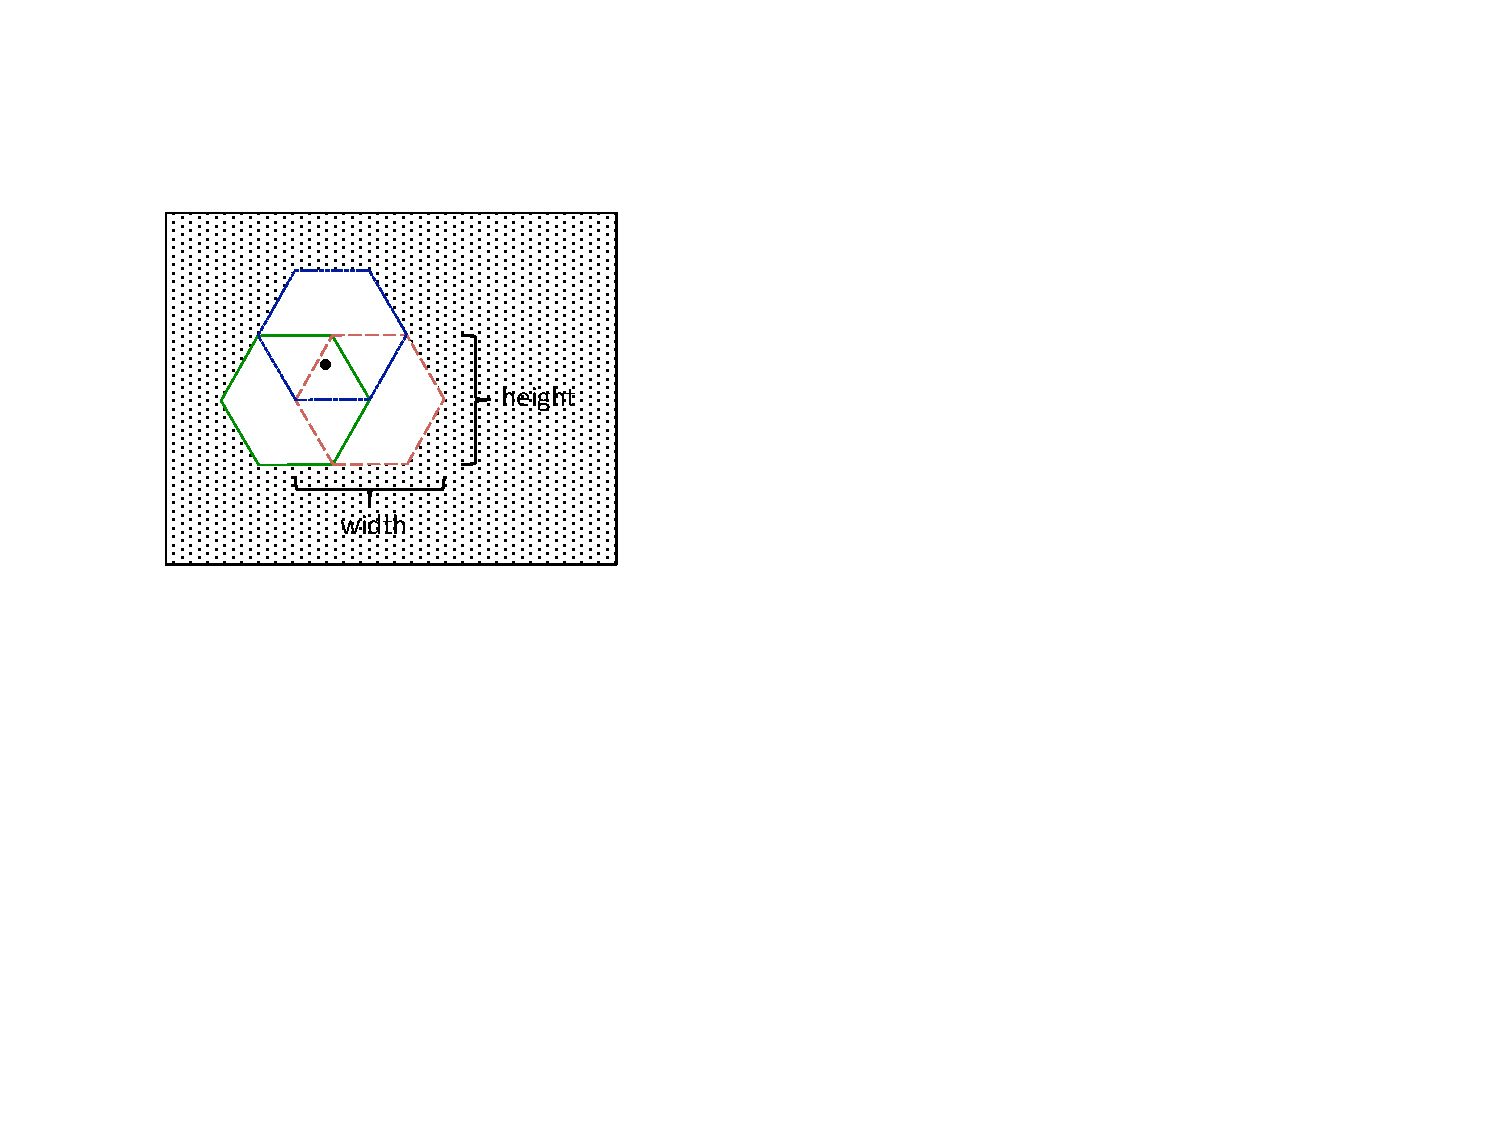
\includegraphics[width=0.2\textwidth]{figs/single_hex.pdf}
%     \caption{Representing a point and radius as three hexagons. The width and height correspond to the radius.}
%  \label{fig:grid}
%\end{figure}

%\begin{figure}
%  \centering
%     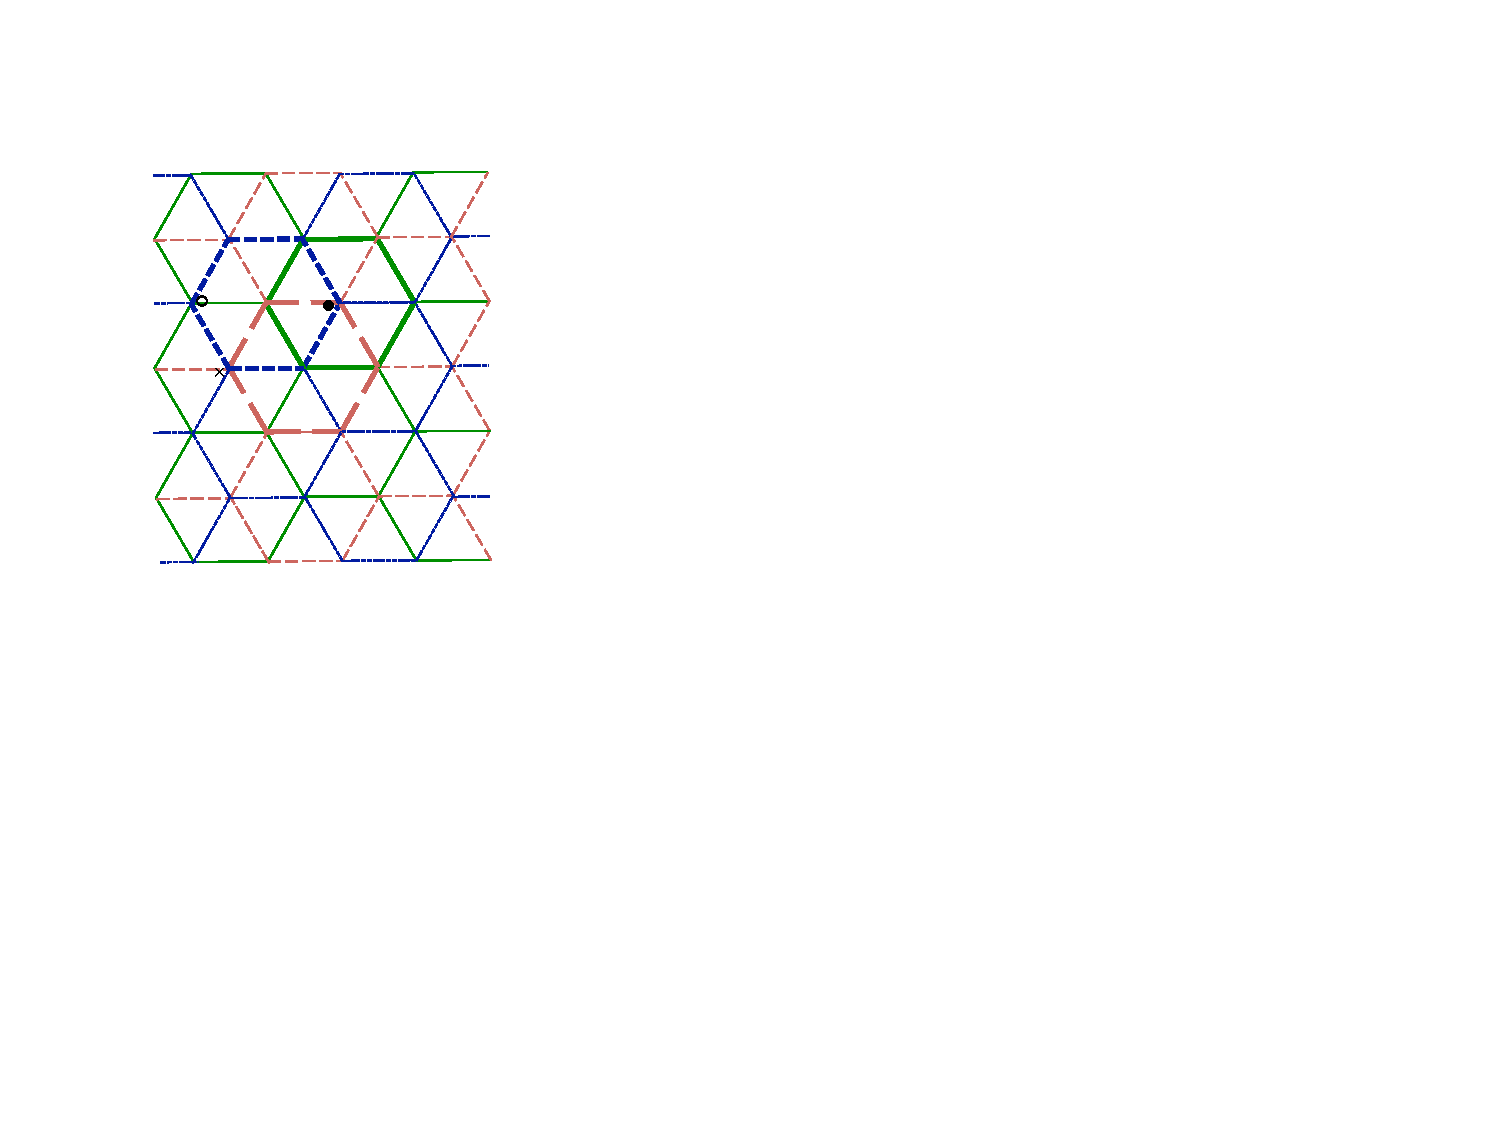
\includegraphics[width=0.25\textwidth]{figs/multiple_hex.pdf}
%     \caption{Overlay of map with multiple hexagons.}
%  \label{fig:grid2}
%\end{figure}

For this dataset, we present results for the following three queries:
\begin{verbatim}
Q1: SELECT COUNT(*) WHERE category="Thai"

Q2: SELECT TOP 10 restaurant
WHERE category="Mexican" AND
(hex2mi=1 OR hex2mi=2 OR hex2mi=3)
ORDER BY stars

Q3: SELECT restaurant, MAX(stars) 
WHERE category="Mexican" OR
category="Chinese" OR category="Indian"
OR category="Greek" OR category="Thai"
OR category="Japanese"
GROUP BY category
\end{verbatim}

Q1 is a count on the number of Thai restaurants.
%In our dataset, we map the category string to an integer id.
%The input domain is 11 bits for this query because there are 900 categories.
Q2 returns the top 10 Mexican restaurants within
a 2 mile radius of a user-specified location by querying three hexagons.
We assume that the provider caches the intermediate table for the 
Top 10 query as described in Section~\ref{sec:topk} because it is a common query.
%The query size is large because the user has to query for restaurants 
%that match one of the three location hexagons.
%The input domain is 22 bits for this query (11 bits for the category and 11 bits for 
%the hexagon id).
Finally, Q3 returns the best rated restaurant from
a subset of categories.
This requires more communication than other queries because 
it performs a MAX with many disjoint conditions, 
as described in Section~\ref{sec:min-max}. Although most queries will probably
not have this many disjoint conditions, we test this query to show
that Splinter's protocol for this case is also practical.

Note that for Q2 and Q3, the communication costs will be higher compared
to Q1 because in Q2 and Q3, 
we are returning ASCII-encoded strings of the restaurant names rather
than just an integer in Q1.

%Although the intermediate table is smaller, the FSS scheme has to process more bits.
%Finally, in this query, the slower multi-party FSS with Paillier 
%and caching previous FSS evaluations during the query are not useful
%because the intermediate table has distinct values for the predicate
%describing the category and location.

\paragraph{Flight search:}
We implement a flight search service similar to Kayak~\cite{kayak}, using 
a public flight dataset~\cite{enigma}. The columns
are flight number, origin, destination, month, delay, and price. To find a flight,
we search by origin-destination pairs. 
We present results for two queries:

\begin{verbatim}
Q1: SELECT AVG(price) WHERE month=3 
AND origin=1 AND dest=2

Q2: SELECT TOP 10 flight_no
WHERE origin=1 and dest=2 ORDER BY price
\end{verbatim}

Q1 shows the average price for a flight during a certain month.
%If we 
%issue this query for every month, we can obtain a histogram of average prices for the year.
%In this query, the input domain is 17 bits (13 bits
%for flight number and 4 bits for the month).
Q2 returns the top 10 cheapest flights for a given source and destination, which 
we encode as integers.
Since this is a common query, the results in Figure~\ref{fig:big-results} 
assume a cached Top 10 intermediate table. 
%This query
%has an input domain of 13 bits.

\paragraph{Map routing:}
We implement a private map routing service, using real traffic map data from DIMACS~\cite{dimacs} for New York City.
However, implementing map routing in Splinter is difficult because the providers can
perform only a restricted set of operations. The challenge is to find a shortest path 
algorithm compatible with Splinter. Fortunately,
%Storing all possible shortest paths requires 
%substantial amounts of storage. For example, 
%storing all shortest paths for New York City requires $2^{36}$ rows! 
%The user could download the map and find the shortest path locally, which
%is bandwidth heavy, and the user would also have to download updates constantly.
extensive work has been done to optimize map routing~\cite{bast2015route}.
One algorithm compatible with Splinter is transit node routing 
(TNR)~\cite{tnr, bast2007fast}, which has been
shown to work well in practice~\cite{bast2009ultrafast}. 
In TNR, the provider divides up a map into grids, 
which contain at least one transit node, i.e. a transit node 
that is part of a "fast" path. There is also a separate table
that has the shortest paths between all pairs of transit nodes, which 
represent a smaller subset of the map. To execute a shortest path query for a given
source and destination, the user can use FSS to download the paths
in her source and destination grid. She locally finds the shortest path to the source transit node
and destination transit node. Finally, she queries the provider for the shortest path
between the two transit nodes.

We used the source code from Arz et al.~\cite{tnr} and identified the 1333 transit nodes. We divided the map into 5000 grids,
and calculated the shortest path for all transit node pairs. The grid table has 5000 rows
representing the edges and nodes in a grid, and the transit node table has about 800,000
rows representing the number of shortest paths for all transit node pairs. 

Figure~\ref{fig:big-results} shows the total response time for a routing query
between a source and destination in NYC. Figure~\ref{fig:map-results} shows
the breakdown of time spent on querying the grid and transit node table.
One observation is that the multi-party version is slightly faster than the two party
version because it is faster at processing the grid query as shown in Figure~\ref{fig:map-results}.
The two-party version of FSS requires using GMP operations, which is slower than integer operations
used in the multi-party version, but the two-party version requires less bandwidth.

\begin{figure}
	\centering
		\begin{tabular}{cccc}
			\toprule
			\bf FSS scheme & \bf Grid & \bf Transit Node & \bf Total \\
			\midrule
			Two Party & 0.35 s  & 0.85 s & 1.2 s \\
			Multi-party & 0.15 s & 0.85 s & 1.0 s \\
			\bottomrule
		\end{tabular}
	\caption[Grid, transit node, and total query times for NYC map.]
	{Grid, transit node, and total query times for NYC map. 
		A user issues 2 grid queries and one transit node query. The two grid queries
		are issued together in one message, so there are a total of 2 network round trips.}
	\label{fig:map-results}
\end{figure}

Splinter has response times of 50 ms to 1.6 seconds. Although these response times are
much higher compared to a system without FSS and Splinter, 
privacy-sensitive users are often willing
to trade some performance for better security. For
example, fetching a website on Tor 
takes 3-4 seconds~\cite{torStats}.
Therefore, we believe that our performance is 
acceptable.

\subsubsection{Communication Costs}
\label{sec:communication}
Figure~\ref{fig:big-results} shows the total bandwidth of a query request and response
for the various case study queries. The sum of those
two values represents total bandwidth between the providers and user.

There are two main observations. First, both the query and response sizes are \textit{much smaller} than the size
of the database in most cases. 
Second, for non-aggregate queries, the multi-party protocol has 
a smaller response size compared to the two-party protocol but the query size is much larger
than the two-party protocol, leading to higher overall communication. 
For aggregate queries, the multi-party FSS scheme is only xor homomorphic, so
it outputs all the matches for a specific predicate/condition. The user has to perform
the aggregation locally, leading to a larger response size than the two-party protocol.
Overall, the multi-party protocols have higher total bandwidth compared to the two-party protocols
despite some differences in response size. However, FSS is a relatively new cryptographic
primitive, especially compared to PIR and garbled circuits, so we believe that
improvements in the FSS protocol could lower these communication costs in the future.

As stated in Section~\ref{sec:splinter_cases}, querying with 
Splinter and PIR systems might be more efficient than
downloading the whole database, assuming that such a download is possible
(no rate limiting or query restrictions). To better quantify
the "break even" point, i.e. where the communication costs are equal
to the database size, we look at our case study datasets.
For two-party Restaurant Q1, it will take about 10,000 of these types of queries
before reaching that point.
For multi-party Restaurant Q1 and two-party Restaurant Q2, it would take about 1000 queries.
For multi-party Restaurant Q2 and Restaurant Q3, 
it would take about 10 queries to reach that point. However, users tend to issue
different kinds of queries and updates might happen, it is not obvious
whether downloading the whole database or using Splinter would be more efficient
for this case study. Moreover, the purpose of this case study is to compare
Splinter's performance on smaller datasets to prior systems and to larger datasets.
For flights, it would take about 550 queries for multi-party Flights Q1 and 
50,000 queries for the other flight queries. Finally, for maps,
it would take 25,000 queries for the two-party version and 2500 for the multi-party
version. However, these two databases are larger
than Yelp and change more frequently, so it might not make sense
to download the database. We discuss Splinter-amenable web services
in more detail in Section~\ref{sec:splinter_cases}.

%\subsection{Impact of caching FSS outputs}
%\label{sec:eval_cache}
%In this section, we evaluate the impact of caching FSS outputs in the same query
%as described in Section~\ref{sec:caching}. One observation is that caching
%has no effect on certain queries, such as the Top-10 and the map routing queries, because
%for the commonly queried predicate column in the table, each record has a distinct value.
%It works well for queries where the predicate column has few distinct values relative to the 
%number of records, such as the restaurant COUNT and flights AVG query described above.
%
%\begin{figure}
%\centering
%\small
%\scalebox{0.85}{
%\begin{tabular}{ccccc}
%\toprule
%\bf Query & \bf FSS scheme & \bf No caching  & \bf Caching & \bf Speedup\\
%\midrule
%\multirow{2}{*}{Restaurant Q1} & Two-Party & 271 ms & 57 ms & 4.8x \\
% & Multi-party & 252 ms & 52 ms & 4.8x\\
%\multirow{2}{*}{Flight Q2} & Two-Party & 14.6 s & 1.5 s & 9.7x \\
%& Multi-party & 50.6 s & 1.6 s & 31.6x \\
%\bottomrule
%\end{tabular}
%}
%\caption{Speed up of queries as a result of caching FSS outputs in the same query.}
%\label{fig:caching-result}
%\end{figure}
%
%Figure~\ref{fig:caching-result} shows some examples of speed ups of queries as a result
%of caching FSS outputs in the same query. For the Yelp query, there were only about 900
%unique categories, so each provider only needed to perform about 900 FSS operations on the 
%database of 225,000 rows per query. 
%For the flight query on average price for a specific flight in a month, 
%there were only about 5000 unique
%source-destination pairs, so each provider only needed to perform about 5000 FSS operations
%per query for a database with 6.1 million rows.]

\subsubsection{Coverage of Supported Queries}
\label{sec:supported_queries}

%\begin{figure}[h]
%\centering
%\scalebox{0.78}{
%\begin{tabular}{c|C{3cm}|c}
%\toprule
%\bf Website & \bf Splinter Primitive & \bf \# of Search Features \\
%\midrule
%\multirow{3}{*}{Yelp} & Equality & 4 \\
%%\midrule
% & Range & 2 \\
%%\midrule
% & Sorting & 4 \\
%\midrule
%\multirow{4}{*}{Hotels.com} & Equality & 3 \\
%%\midrule
% & Range & 3 \\
%%\midrule
% & Sorting & 4 \\
% & Not supported & 1 \\
%\midrule
%\multirow{3}{*}{Kayak} & Equality & 4 \\
%%\midrule
% & Range & 4 \\
%%\midrule
% & Not supported & 1 \\ 
%\midrule
%Google Maps & Equality & 3 \\
%\bottomrule
%\end{tabular}
%}
%\caption{Example websites and the number of search features supported by Splinter for a given primitive.}
%\label{fig:websites}
%\end{figure}


\begin{figure}
	\centering
		\begin{tabular}{c|c|c}
			\toprule
			\bf Website & \bf Search Feature & \bf Splinter Primitive \\
			\midrule
			\multirow{3}{*}{Yelp} & Booking Method, Cities, Distance & Equality \\
			%\midrule
			& Price & Range \\
			%\midrule
			& Best Match, Top Rated, Most Reviews & Sorting \\
			& Free text search & --- \\
			\midrule
			\multirow{4}{*}{Hotels.com} & Destination, Room type, Amenities & Equality \\
			%\midrule
			& Check in/out, Price, Ratings & Range \\
			%\midrule
			& Stars, Distance, Ratings, Price & Sorting \\
			%\midrule
			& Name contains & --- \\
			\midrule
			\multirow{2}{*}{Kayak} & From/To, Cabin, Passengers, Stops & Equality \\
			%\midrule
			& Date, Flight time, Layover time, Price & Range \\
			%\midrule
			\midrule
			Google Maps & From/To, Transit type, Route options & Equality \\
			\bottomrule
		\end{tabular}
	\caption{Example website search features and their equivalent Splinter query class.}
	\label{fig:websites}
\end{figure}

We also manually characterized the applicability of Splinter to several widely used online services by studying how many of the search fields on these services' interfaces Splinter can support.
Figure~\ref{fig:websites} shows the results. 
Most services use equality and range predicates: for example, the
Hotels.com user interface includes checkboxes for selecting categories, neighborhoods, stars, etc, a range fields for price, and one free-text search field that Splinter does not support.
In general, all features except free-text search could be supported by Splinter.
For free-text search, simple keywords that map to a category (e.g., ``grocery store'') could also be supported.

\subsubsection{Comparison to Other Private Query Systems}
\label{sec:comparison}

\begin{figure}
	\centering
	\begin{tabular}{lcc}
		%\multicolumn{3}{c}{Round Trips (RTs) Required}\\
		\toprule
		\bf Splinter Query & \bf RTs in~\cite{goldberg} & \bf RTs in Splinter \\
		\midrule
		Restaurant Q1 & 6 & 1 \\
		\midrule
		Restaurant Q2 & 6 & 1 \\ 
		\midrule
		Restaurant Q3 & 6 & 11 \\
		\midrule
		Flights Q1 & 13 & 1 \\
		\midrule
		Flights Q2 & 8 & 1 \\
		\midrule
		Map Routing & 19 & 2 \\
		\bottomrule
	\end{tabular}
	\caption{Round trips required in Olumofin et al.~\cite{goldberg} and Splinter.\protect\footnotemark}
	\label{fig:rt-comparison}
\end{figure}

\begin{figure}
	\centering
	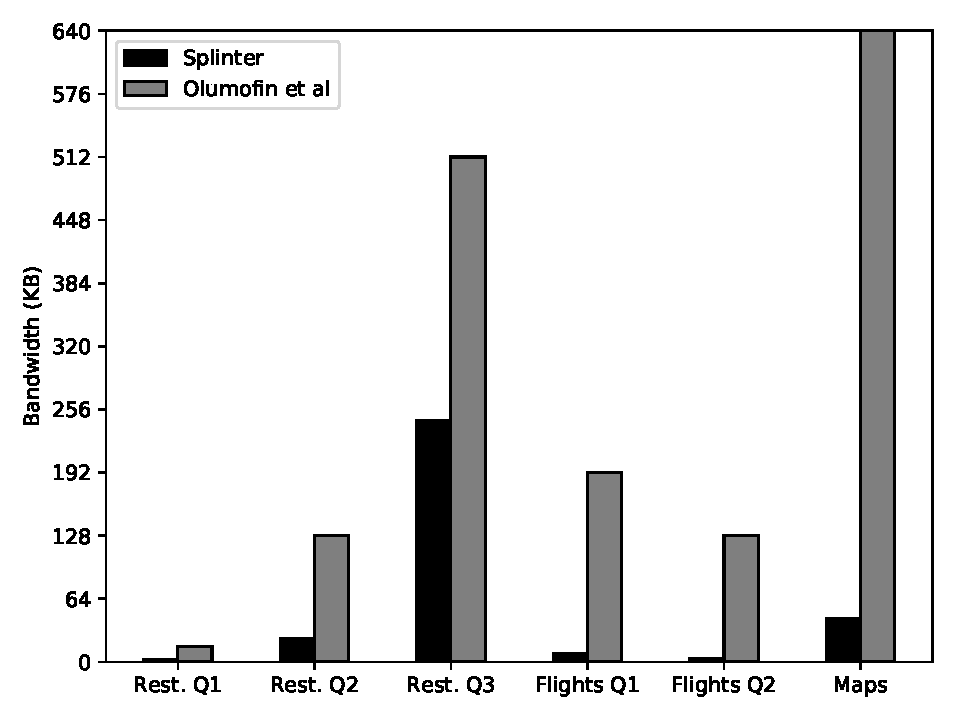
\includegraphics[width=\textwidth]{splinter-figs/bandwidth_comparison.pdf}
	\caption{Total bandwidth for Splinter and Olumofin et al.~\cite{goldberg}}
	\label{fig:bandwidth_comp}
\end{figure}

\footnotetext{
	The number of round trips in Restaurant Q3 is $O(\log n)$ in both Splinter and Olumofin et al., but the absolute number is higher in Splinter because we use a binary search whereas Olumofin et al.~use a 4-ary tree. Splinter could also use a 4-ary search to achieve the same number of round trips, but we have not yet implemented this.}

\begin{figure}
	\centering
	\begin{tabular}{lcc}
		%\multicolumn{3}{c}{Round Trips (RTs) Required}\\
		\toprule
		\bf Splinter Query & \bf Time in~\cite{goldberg} & \bf Time in Splinter \\
		\midrule
		Restaurant Q1 & 80 ms & 40 ms \\
		\midrule
		Restaurant Q2 & 245 ms & 130 ms \\ 
		\midrule
		Restaurant Q3 & 1.2 s & 1.1 s \\
		\midrule
		Flights Q1 & 10.9 s & 0.97 s \\
		\midrule
		Flights Q2 & 150 ms & 15 ms \\
		\midrule
		Map Routing & 10.6 s & 1.1 s \\
		\bottomrule
	\end{tabular}
	\caption{Server-side computation costs for Olumofin et al.~\cite{goldberg} and Splinter.}
	\label{fig:serverside-comparison}
\end{figure}

To the best of our knowledge, the most recent
private query system that can perform a similar class of queries
as Splinter is that of Olumofin et al.~\cite{goldberg},
which uses multi-party PIR. In PIR, a user can query for an index $i$
without revealing the index or the result to the servers, making 
it a more restrictive querying model compared to FSS, but Olumofin et al.
develops protocols to extend PIR beyond just index querying. However,
FSS can perform many of the complex queries in Olumofin et al.
without additional protocols, such as COUNT and SUM 
with non-index predicates.

We implemented the private query protocol in Olumofin et al., ported our
case queries, and ran them on the same Amazon AWS setup as Splinter
(described at the beginning of this section).
We compare the two-party version of Splinter with Olumofin et al.
because the system of Olumofin et al. assumes only two parties 
and does not describe how to extend it to more servers.
\footnote{From our understanding, it is possible for Olumofin et al. to support
	more than two parties, but server-side computation and bandwidth would increase, 
	most likely eliminating effects of the optimizations described in their paper.}
In particular, we compare Olumofin et al. and Splinter on
the following three metrics: number of  
round trips, bandwidth, and server-side computation. We find
that across all of our queries, Splinter is almost always 
more efficient than Olumofin et al., often by an order of 
magnitude or more.

Figure~\ref{fig:rt-comparison} shows 
the round trips required in Olumofin et al.'s system and in Splinter
for the queries in our case studies. Olumofin et al. creates
an $m$-ary ($m=4$) B+ index tree for the dataset and
uses PIR to extract the results. Consequently, their queries
require $O(\log_m n)$ round trips, where $n$ is
the number of records. In Splinter, the number of rounds trips
does not depend on the size of the database for most queries.
As shown in Section~\ref{sec:complex-aggregates}, 
the exception is for MIN/MAX and TOPK queries with many disjoint
conditions where Splinter's
communication is similar; if there are a small number of disjoint
conditions, Splinter will be faster than previous systems 
because the user can issue parallel queries.

Figure~\ref{fig:bandwidth_comp} shows the total bandwidth
required in Olumofin et al.'s system and in Splinter. Note that
Olumofin et al. does not have a direct way to support queries with
disjoint OR conditions used in Restaurant Q3, so we assumed that they issue a separate query
for each OR condition. Splinter has much lower overall communication
costs, especially for the queries on the larger flights and maps
databases. The main reason for this is that the bandwidth
in PIR depends on both the number of database records (specifically a square root factor) 
and record size whereas in FSS, the bandwidth is
independent of the number of records and depends just on the record size. 
Therefore, the disparity in bandwidth
will increase as the database size increases. This larger bandwidth
is problematic on mobile networks where data is more expensive.

Figure~\ref{fig:serverside-comparison} shows the server-side computation
costs for both systems. As expected, the difference is minimal 
on the smaller restaurant database but greater on the larger databases. 
Although the PIR scheme used in Olumofin et al. has similar performance to
FSS, their protocols require more PIR operations per record.

Compared to Splinter, Olumofin et al. also has more round trips
for the smaller database, which increases the overall response times. For example,
in our experimental setup with 14 ms network latency, Olumofin et al. would 
incur an additional 70 ms delay versus Splinter for Restaurant Q1 and Restaurant Q2. 
This delay increases as we move to mobile networks. If we replace
the client with a mobile device on a 4G network with 
latency of approximately 100 ms~\cite{mobile-delays}, 
the restaurant queries would incur an additional 500 ms delay in Olumofin et al.
compared to Splinter. For bigger databases, the number of round trips increases,
so the total amount of latency incurred will also increase. For instance,
for maps, the additional latency on Olumofin et al. would be about 1.7 seconds.

%Finally, the system in~\cite{goldberg} has weaker security guarantees:
%it requires \textit{all} the providers to be honest, whereas Splinter
%only requires that \textit{one} provider is honest.

%\begin{figure}
%\centering
%\scalebox{0.9}{
%\begin{tabular}{lcc}
%\multicolumn{3}{c}{Bytes Transferred}\\
%\toprule
%\bf Splinter Query & \bf \cite{goldberg} & \bf Splinter \\
%\midrule
%Restaurant Q1 & 3-30 KB & 1 \\
%\midrule
%Restaurant Q2 &  & 1 \\ 
%\midrule
%Flights Q1 & 22 & 1 \\
%\midrule
%Flights Q2 & 12 & 1 \\
%\midrule
%Map Routing & 19 & 2 \\
%\bottomrule
%\end{tabular}
%}
%\caption{For the queries in our evaluation, we show the estimated difference in round trips between Olumofin et al.~\cite{goldberg} and Splinter.}
%\label{fig:comparison}
%\end{figure}


\subsubsection{FSS Microbenchmarks}
\label{sec:micro}
Cryptographic operations are the main
cost in Splinter.
We present microbenchmarks to show these costs of various
parts of the FSS protocol, 
tradeoffs between various FSS protocols,
and the throughput of FSS. The microbenchmarks
also show why the response times in Figure~\ref{fig:big-results} 
are different between the two-party and multi-party FSS cases.
All of these experiments are done on one core to show the 
per-core throughput of the FSS protocol.

\paragraph{Two-party FSS:}
For two-party FSS, generating a function share takes less than 1 ms.
The speed of FSS evaluation is proportional to the size of the input domain, i.e. number of bits per record. 
We can perform around 700,000 FSS evaluations per second on
24-bit records, i.e. process around 700,000
distinct 24-bit records, using one-way compression functions.
Figure~\ref{fig:micro2} shows the per-core throughput of our implementation
for different FSS schemes, i.e. number of unique database records that can be processed
per second. It also shows that using one-way compression functions
as described in Section~\ref{sec:fastfss}, we obtain a $2.5\times$ speedup over using 
AES as a PRG.

\begin{figure}
	\centering
	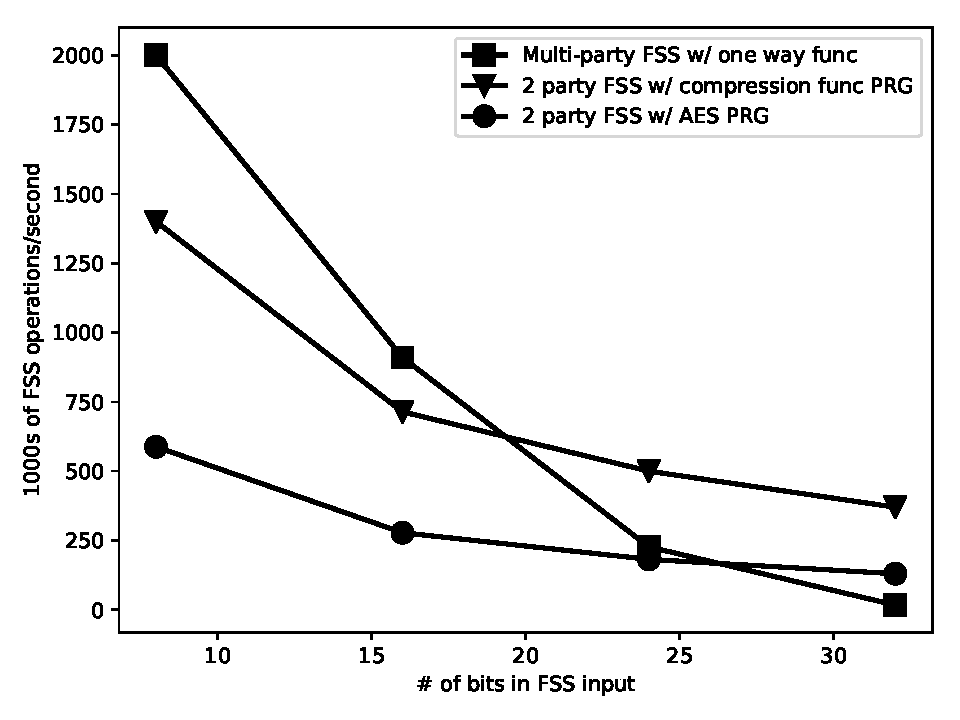
\includegraphics[width=\textwidth]{splinter-figs/micro.pdf}
	\caption[Per-core throughput of various FSS protocols.]{Per-core throughput of various FSS protocols. 
		The graph shows the number of FSS operations that can be performed, i.e. database records processed, per second for various input sizes, on one core.}
	\label{fig:micro2}
\end{figure}


\paragraph{Multi-party FSS:}
As shown in Figure~\ref{fig:micro2}, for the multi-party FSS 
scheme from~\cite{fss},
the time to generate the function share and evaluate it is proportional
to $2^{n/2}$ where $n$ is the number of bits in the input domain. 
The size of the share scales with $2^{n/2}$
rather than just $n$ in the two-party case. 
An important observation is that using one-way compression 
functions instead of AES does not make a significant difference for multi-party 
FSS because the PRG is called less often compared to two-party FSS. 
For small input domains ($<$ 20 bits), 
the multi-party version of FSS is faster than the 2-party version, but 
a provider cannot aggregate locally for SUM and COUNT queries in the multi-party version.
%However, for smaller input domains, at the
%cost of additional bandwidth for increased function share size, she will receive faster execution and
%more security by being able to split her shares.

%\begin{figure}
%	\centering
%		\begin{tabular}{cC{2.7cm}C{3cm}}
%			\multicolumn{3}{c}{Time to generate function shares} \\
%			\toprule
%			\bf \# of bits & \bf Query Gen in Boyle et al~\cite{fss} & \bf Query Gen in Riposte~\cite{corrigan-gibbs:riposte}\\
%			\midrule
%			8 & $<$ 1 ms  & 0.06 s \\
%			16 & $<$ 1 ms & 1 s \\
%			24 & 44 ms & 16 s \\
%			32 & 166 ms & 265 s \\
%			\bottomrule
%		\end{tabular}
%	\caption{Query generation times for multi-party FSS schemes using one-way functions~\cite{fss} and
%		using Paillier~\cite{corrigan-gibbs:riposte}.}
%	\label{fig:mp_querygen}
%\end{figure}
%
%For the scheme from~\cite{corrigan-gibbs:riposte}, which uses Paillier encryption, generating
%a function share is slower compared to~\cite{fss} because 
%it requires many exponentiations over a large integer group and 
%depends on the number of record bits. Figure~\ref{fig:mp_querygen} 
%shows a summary of the query generation times
%for both schemes. However, the 
%evaluation of the function share is independent of the size of
%the input domain. The output of the function share in~\cite{corrigan-gibbs:riposte}
%returns a group element that is additive in a large integer group, but in
%order to have this property, the performance is lower compared to~\cite{fss}.
%We can perform 250 FSS evaluations a second, but this lower performance 
%is useful for SUM and COUNT operations on bandwidth-constrained clients.

\subsubsection{Hosting Costs}
\label{sec:pricing}
We estimate Splinter's server-side computation cost on Amazon AWS, 
where the cost of a CPU-second using Amazon Lambda is about 0.005 cents. 
The cost of storage and running a web server can be amortized over requests.
We found that most of our queries cost less than 0.005 cents. Map queries are a bit more costly,
about 0.05 cents to run a shortest path query for NYC, because the amount of 
computation required is higher. With the decreasing cost of cloud computing resources~\cite{decrease-aws},
we expect even lower costs in the future. Although there are other costs associated with running a web service,
our results show that Splinter's server-side computation costs are very reasonable.
%Costs for Amazon AWS and other cloud services have been decreasing because
%of innovation and competition~\cite{aws-decreasing}, and further improvements to the FSS protocol
%could also reduce costs. Therefore, we expect our costs per query to decrease over time.


\subsection{Discussion and Limitations}
\label{spl-sec:discussion}

\paragraph{Economic feasibility:}
\label{sec:disc-economics}

Although it is hard to predict real-world deployment, we believe that Splinter's low cost makes it economically feasible for several types of applications.
Here are some possible methods for monetization.
For example, despite many current data owners, such as Yelp and Google Maps, generating revenue primarily by showing ads and mining user data,
they can license their data to Splinter providers and have these providers manage a Splinter deployment. The providers
can then charge a subscription fee, e.g. \$1 a month, for usage of the server.
Similarly, these providers can collectively issue a utility token that
can be used to pay for the queries.
Splinter's trust model, where only one provider needs to be honest, also makes 
it easy for new providers to join the market, increasing users' privacy.

This business model seems reasonable as studies have shown that 
many consumers are willing to pay for services that protect their privacy~\cite{atlantic,atlantic2}. 
In fact, users might not use certain services because of privacy concerns~\cite{ravichandran2009capturing,riley2008tolls}.
Similarly, more users are using sites like DuckDuckGo and technologies like Tor 
because they are unwilling to have sites track their
query behavior, which shows a growing consumer market for privacy-preserving technologies. 
However, whether such a business model would work or be feasible 
in practice is beyond the scope of this dissertation.
%Well-known sites like OkCupid, Pandora, Youtube, and Slashdot allow users to 
%pay a monthly fee to remove ads that collect their information, showing there is
%already a demographic willing to pay for privacy. Moreover,

%As shown in Section~\ref{sec:pricing}, the cost of running queries on Splinter is low, with our most expensive query, map routing, costing less than 0.005 cents in AWS resources.
%At this cost, providers could offer Splinter-based map routing for a subscription fee of \$1 per month.
%Moreover, the availability of techniques like Splinter might make it easier to introduce 
%regulation about privacy in certain settings, similar to current privacy regulations in HIPAA~\cite{hipaa}
%and GDPR~\cite{gdpr}.

%Nonetheless, there are already successful open databases containing most of the data in these services, such as OpenStreetMap~\cite{osm}, and basic data on locations does not change rapidly once collected.
%There are already multiple Android and iOS applications that download subsets of OpenStreetMap data for  offline routing and update it periodically~\cite{osm-offline}.

%\subsection{Extensions to Splinter}
%\label{sec:disc-extensions}
%
%To support more workloads, Splinter's query model and evaluation algorithms can be extended in several ways.

%Finally, Splinter does have some limitations.
%First, FSS, like PIR, requires scanning the whole input dataset on
%every query, to prevent providers from figuring out which records have
%been accessed.
%Second, Splinter does not support some SQL features, such as private join conditions.
%Despite these limitations, we show that Splinter is practical on large
%real-world datasets, such as maps, and can support many of today's online applications.
%Because human-created datasets are unlikely to grow faster than
%hardware capabilities in the future, we believe Splinter's techniques will only
%become more practical over time.

\paragraph{Unsupported queries:}
As shown in Section~\ref{sec:querymodel}, Splinter supports only a subset of SQL.
Splinter does not support partial text matching or image matching, which are common in types of applications
that might use Splinter. Moreover, Splinter cannot support private joins, i.e. Splinter can only support joining with 
another table if the join condition is public, which encompasses a large majority of join operations. 
Despite these limitations, our study in Section~\ref{sec:supported_queries} 
shows Splinter can support many application search interfaces.

\paragraph{Number of providers:} 
One limitation of Splinter is that 
a Splinter-based service has 
to be deployed on at least two providers. 
However, previous practical PIR systems described in Section~\ref{spl-sec:related}
also require at least two providers. 

%Unlike those systems, 
%Splinter requires only \textit{one} honest provider whereas those systems
%require \textit{all} providers be honest. Moreover,
%current multi-party FSS schemes do not scale well past 
%three providers, but we believe that further research will improve its efficiency.

%\paragraph{Joins:}
%As shown in Section~\ref{sec:querymodel}, Splinter can support only joining with another table 
%if the join condition is public,
%i.e. the join condition cannot contain sensitive or private information. To do this, 
%providers can run the join before filtering the data using the private condition.
%We leave the development of private join conditions to future work.

\paragraph{Full table scans:}
FSS, like PIR, requires scanning the whole input dataset on every Splinter query,
to prevent providers from figuring out which records have been accessed. 
Despite this limitation, we have shown that Splinter is practical
on large real-world datasets, such as maps.

Splinter needs to scan the whole table only for conditions 
that contain sensitive parameters.
For example, consider the query:
\begin{verbatim}
SELECT flight from table WHERE src=SFO 
AND dst=LGA AND delay < 20
\end{verbatim}
If the user does not consider the delay of 20 in this query to be
private, Splinter could send it in the clear.
The providers can then create an intermediate
table with only flights where the delay $<$ 20 and apply the private
conditions only to records in this table.
In a similar manner, users querying geographic data may be willing to
reveal their location at the country or state level but would like to
keep their location inside the state or country private.

%\paragraph{Maintaining consistent data views:}
%Splinter requires that each provider executes a given user
%query on the same copy of the data. 
%Much research in distributed systems has focused on ensuring
%databases consistency across multiple providers~\cite{spanner, ongaro:raft, tu:silo}.
%Using the appropriate consistency techniques is dependent
%on the application and an active area of research.
%Applying those techniques in Splinter is beyond the scope
%of this dissertation.

\subsection{Related Work}
\label{spl-sec:related}
Splinter is related to work in Private Information Retrieval (PIR),
garbled circuit systems, encrypted data systems, 
and Oblivious RAM (ORAM) systems. Splinter achieves higher performance than these systems 
through its mapping of database queries to the Function Secret Sharing (FSS) primitive.

\paragraph{PIR systems:}
Splinter is most closely related to systems that use Private
Information Retrieval (PIR)~\cite{chor1998private} to query a database privately.
In PIR, a user queries for the $i^\mathrm{th}$ record in the database, and the database
does not learn the queried index $i$ or the result.
Much work has been done on improving 
PIR protocols~\cite{ostrovsky2007survey, olumofin2011revisiting}. 
Work has also been done to extend PIR to return multiple records~\cite{groth2010multi},
but it is computationally expensive.
Our work is most closely related to the system in~\cite{goldberg}, which implements
a parametrized SQL-like query model similar to Splinter using PIR, but requires
more computation than Splinter.

Popcorn~\cite{popcorn} is a media delivery service that 
uses PIR to hide user consumption habits from the provider
and content distributor. However, Popcorn is optimized for
streaming media databases, like Netflix, which have a small number (about 8000)
of large records, so Popcorn serves a different purpose than Splinter.

%The systems above have a weaker
%security model: \textit{all} the providers need to be honest.
Note that both systems above are designed and optimized, assuming
two servers, and it is not obvious that these optimizations hold beyond two servers.
Splinter can efficiently support two and three servers because it 
extends Function Secret Sharing (FSS)~\cite{fss,gilboa2014distributed}, which 
enables executions of complex operations such as SUMs in one round trip.

\paragraph{Garbled circuits:}
Systems such as Embark~\cite{lan2016embark}, BlindBox~\cite{blindbox}, 
and private shortest path computation systems~\cite{wu2016}
use garbled circuits~\cite{Yao, goldwasser1997multi} to perform private computation
on a single untrusted server.
Even with improvements in practicality~\cite{bellare2013efficient}, these
techniques still have high computation and bandwidth costs for queries on
large datasets because a new garbled circuit has to be generated for each query.
(Reusable garbled circuits~\cite{goldwasser:sfe} are not yet practical.)
%For example, the recent map routing system by Wu et al.~\cite{wu2016} uses garbled circuits and 
%has $100\times$ higher response time and $10\times$ higher bandwidth cost
%than Splinter.

\paragraph{Encrypted data systems:}
Systems that compute on encrypted data, like 
CryptDB~\cite{popa:cryptdb}, Mylar~\cite{popa:mylar}, SPORC~\cite{feldman:sporc},
Depot~\cite{mahajan:depot}, and SUNDR~\cite{li:sundr}, all try to protect
private data against a server compromise, which is a different
problem than what Splinter tries to solve. CryptDB is most similar to Splinter 
because it allows for SQL-like queries over encrypted data. However, all
these systems protect against a single, potentially compromised server 
where the user is storing data privately, but they do not hide data access patterns. 
In contrast, Splinter hides data access patterns and a user's query parameters 
but is only designed to operate on a cleartext 
datasets that is hosted at multiple providers.


\paragraph{ORAM systems:}
Splinter is also related to systems that use Oblivious RAM~\cite{stefanov:path-oram, lorch2013shroud}. 
ORAM allows a user to read and write data on an untrusted server without
revealing her data access patterns to the server. However, ORAM cannot be easily applied
into the Splinter setting. One main requirement of ORAM is that the user
can only read data that she has written. 
In Splinter, the provider hosts a cleartext dataset, not created by any specific user, 
and many users need to access the same dataset.

\subsection{Conclusions}
\label{spl-sec:conclusion}
Splinter is a new private query system that protects sensitive parameters
in SQL-like queries while scaling to realistic applications. Splinter uses and extends a recent
cryptography primitive, Function Secret Sharing (FSS),
allowing it to achieve much better
performance compared to previous private query systems. We develop
protocols to execute complex queries
with low computation and bandwidth. As a proof of concept,
we have evaluated Splinter with three sample applications---a Yelp clone,
map routing, and flight search---and showed
that Splinter has low response times from 50 ms to 1.6 seconds with low
hosting costs.
